\chapter{Mod�lisation}

\begin{figure}[h]
  \centering
  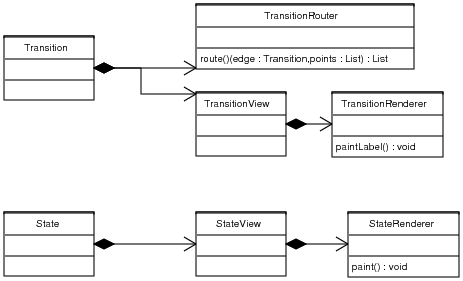
\includegraphics[width=16cm]{img/Affichage.png}
  \caption{Fonctionnement du module d'affichage}
  \label{fig:affichage}
\end{figure}

\begin{figure}[h]
  \centering
  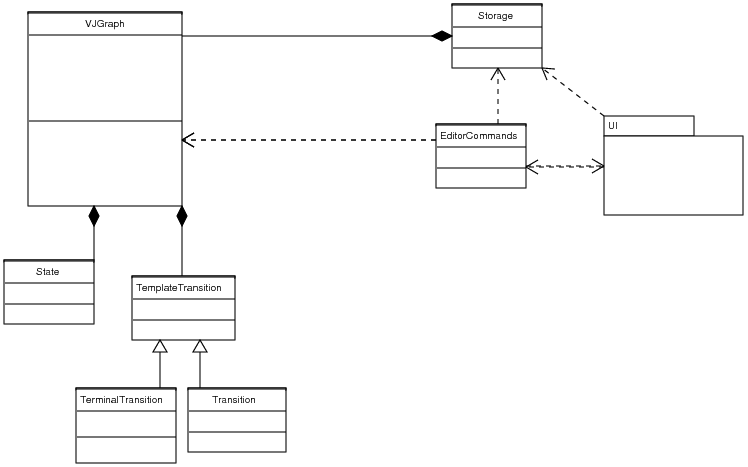
\includegraphics[width=16cm]{img/Overview.png}
  \caption{Vue g�n�rale du programme}
  \label{fig:overview}
\end{figure}

\begin{figure}[h]
  \centering
  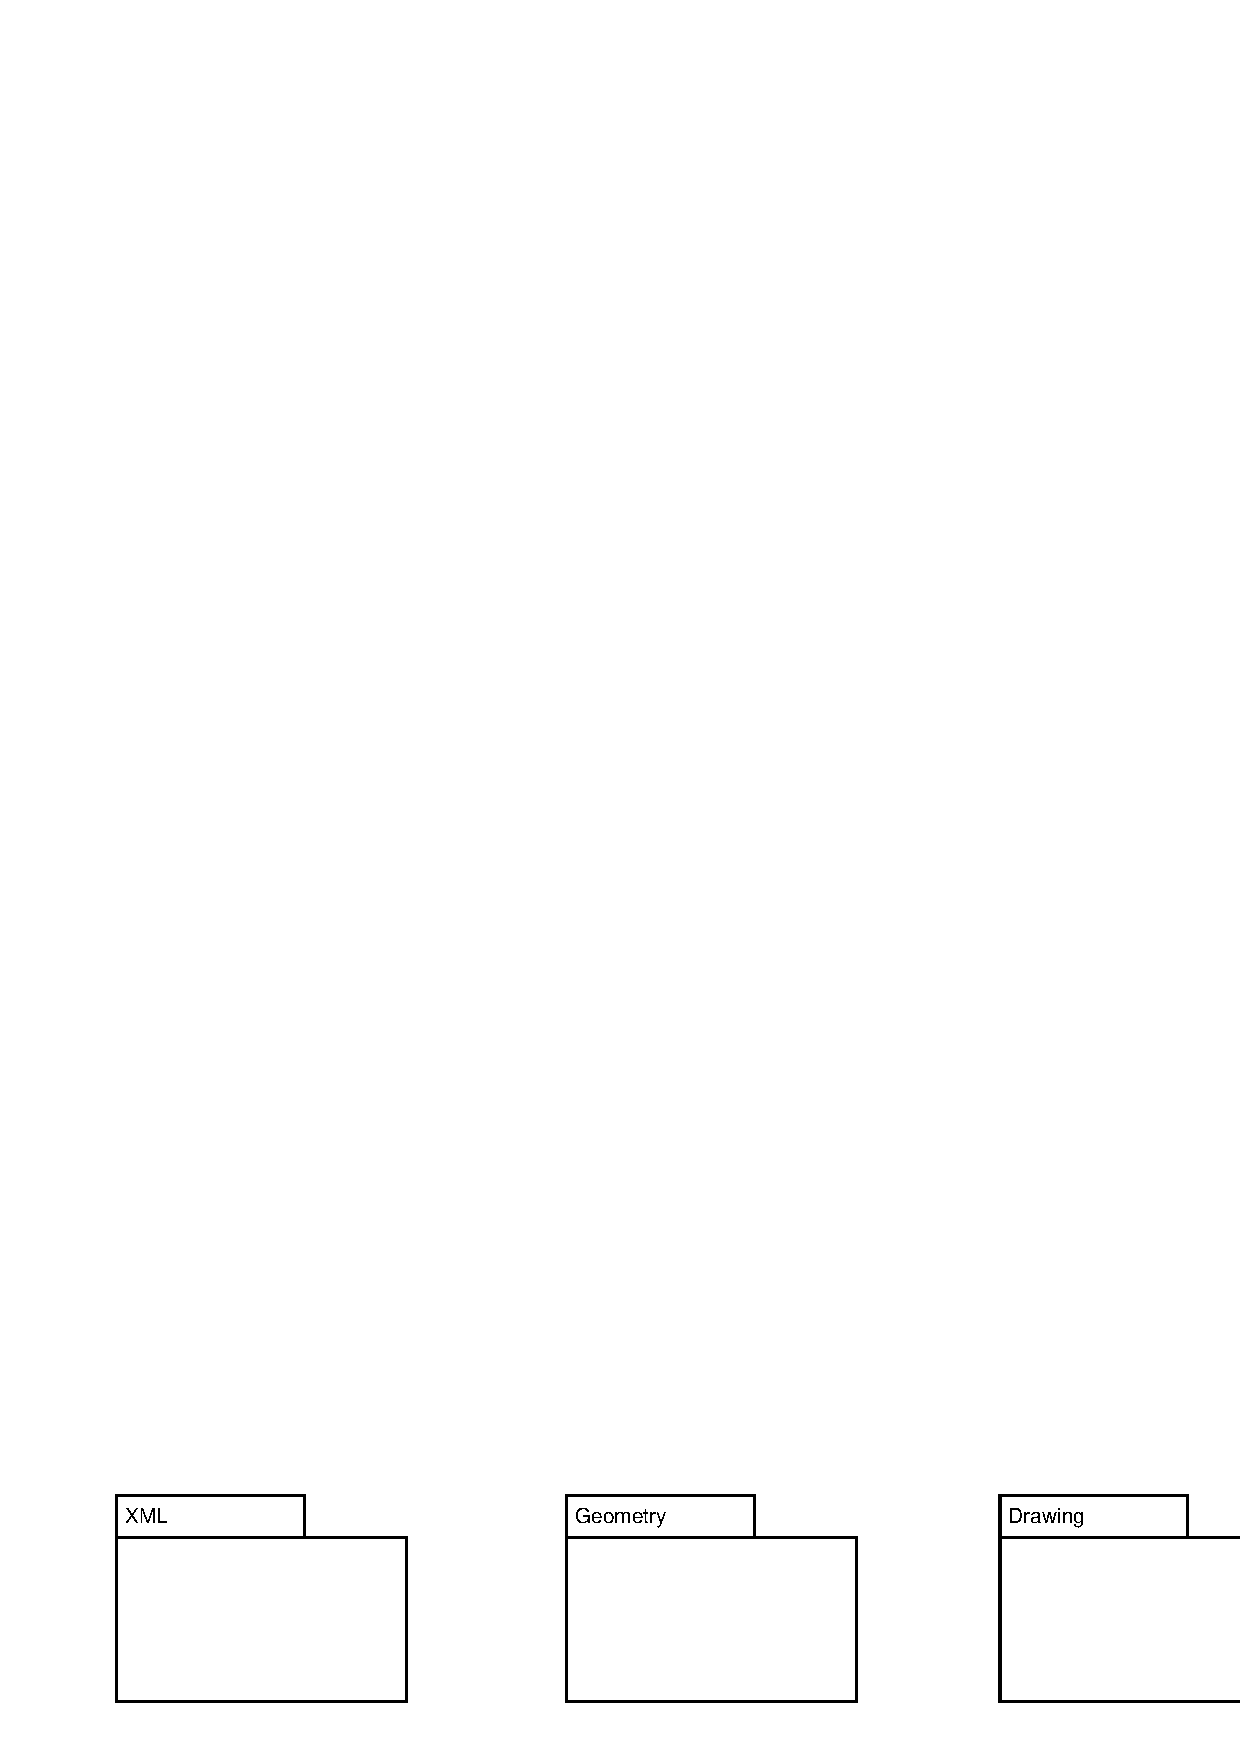
\includegraphics[width=16cm]{img/Packages.png}
  \caption{Mod�lisation des packages}
\end{figure}

\begin{figure}[h]
  \centering
  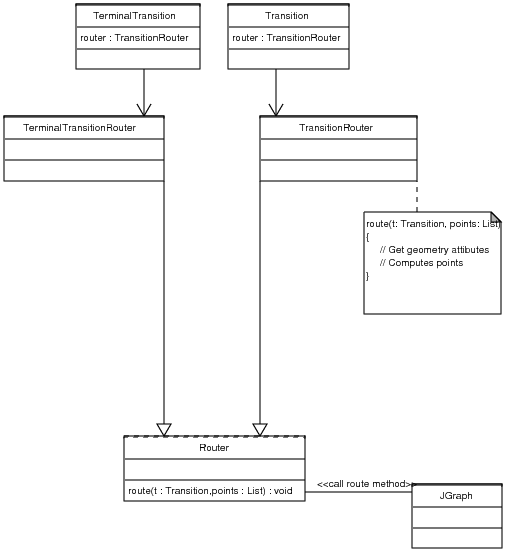
\includegraphics[width=16cm]{img/routing.png}
  \caption{Module d'affichage: Routage des transitions}
  \label{fig:router}
\end{figure}

\chapter{Screenshots}

\begin{figure}[h]
  \centering
  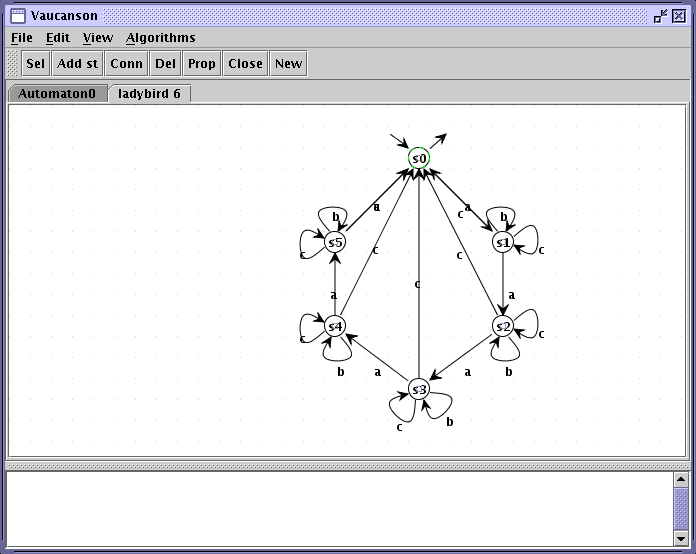
\includegraphics[width=12cm]{img/ui.png}
  \caption{Fen�tre principale}
  \label{fig:ui}
\end{figure}

\begin{figure}[h]
  \centering
  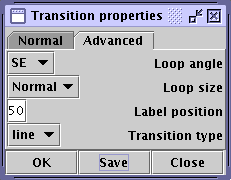
\includegraphics[width=6cm]{img/transition.png}
  \caption{Fen�tre des propri�t�s d'une transition}
  \label{fig:ui_prop}
\end{figure}

\begin{figure}[h]
  \centering
  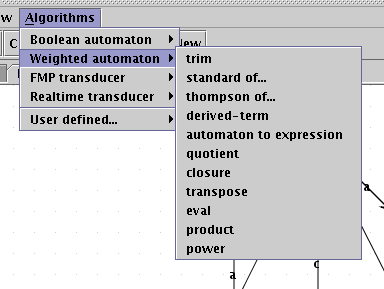
\includegraphics[width=8cm]{img/menu.png}
  \caption{Le menu des algorithmes disponibles}
  \label{fig:algo_menu}
\end{figure}

\chapter{Documentation}
\label{doc}
\section{Modules}

In this section, the directory hierarchy will be described. Some
informations about what does a module will be given too.

Now, VGI is composed of two packages: vgi and vgitoolkit.
\begin{itemize}
\item The vgi package contains the user interface, the code that manage the
interaction between the user, the graphical interface and vgitoolkit.

\item The vgitoolkit contains the geometry and drawing modules, a module
extending the graph class of JGraph to meet our requirements, and some
code translating geometry and drawing properties to JGraph
instructions.
\end{itemize}


\subsection[src/vgi]{VGI package}

In this directory can be found all classes for the user interface, and
some related tools.

\begin{itemize}
\item VGI.java: contains the main function, and creates the editor
  main window.

\item Storage.java: manages informations between the user interface
  and JGraph object. In it exist functions which allow us to find the
  corresponding JGraph object of a panel, or the corresponding XML
  file of a panel. If a algorithm is call by the user, this class
  selects the correct binary following the automaton type.

\item EditorCommands.java: contains utility functions like creating a
  new graph, state or transition. It performs action user required on
  JGraph object.

\item IO.java: contains utility code to call executables, give them
  some input and send output back to VGI.

\item StateProperties.java and TransitionProperties.java: contain the
  user interface for editing geometry and drawing properties of states
  and transitions.
\end{itemize}


\subsection[src/vgitoolkit/vaucanson/vgitoolkit]{VGIToolkit package}

This package contains our graph model for JGraph, utilities for
loading and saving to the XML format. It contains too the geometry and
drawing modules.

\subsubsection{VJGraph}

VJGraph extends the JGraph class to meet our requirements, i.e add
some functionalities to the graph class (JGraph) to become an
automaton class (VJGraph).

Three classes have been created: VJGraph, State and Transition.
Each class contain a geometry and drawing maps.
VJGraph contains informations on the automaton type.
State contains informations on its final and initial transitions.
Transition contains informations on its label and how to display it
following the type of the automaton.

\subsubsection{Geometry module}

The Geometry module is composed of the following classes:
GeometryProperties, GeometricUtilities, and all layout classes.

\paragraph{Geometry Properties:}

This class defines functions to retrieve and set geometry properties
from State or Transition. It enforces the correctness of the given
value and defines some defaults values if nothing was define in the
XML file.

\paragraph{Layouts:}

The goal of layout classes is to provide a nice embedding to the graph.

Layout classes are use to set the location of each states of a
graph. A layout is applied by calling its \emph{apply} method. A
utility class, LayoutTemplate, which all layouts extend, is given. It
defines standard methods for retrieving selected states.

For the time being, layouts only define position of states. But place
has been left so they can modify the geometry properties of
transitions too. TemplateLayout provide a default implementation of a
method which set geometry properties of transitions.

Finally, LayoutTemplate provides a special method to translate the
geometry properties of a set of states to JGraph instructions.

\paragraph{GeometricUtilities:}

This class contains some utility functions, as finding a free angle on
a state for a transition, bezier calculations and so on.


\subsubsection{Drawing module}

\paragraph{Drawing Properties:}

This class is just the same than GeometryProperties but for drawing
properties.

\subsubsection{XML}

Three classes are defined XMLConverter, XMLReader and XMLWriter.

\begin{itemize}
\item XMLConverter: converts a VJGraph object to DOM representation
  and vice-versa.
\item XMLReader: abstraction for reading from a file or string.
\item XMLWriter: abstraction for writing to a file or string.
\end{itemize}


\subsubsection{Translation to JGraph}

As said before the translation of geometry properties of states to
JGraph is done after applying a layout.
The rest of the properties, either geometric or drawing properties,
are translated in different classes. Here is a list of them, each
entry describes what it translates:

\begin{itemize}
\item Router: transition's geometric properties are translated in
  classes TransitionRouter, LoopRouter and TerminalTransitionRouter
  (see Figure \ref{diaroute}).
\item StateView: this class translates drawing properties of states.
\item TransitionView: here is translated drawing AND geometric
  properties of transitions.
\end{itemize}

\begin{figure}[h]
  \centering
  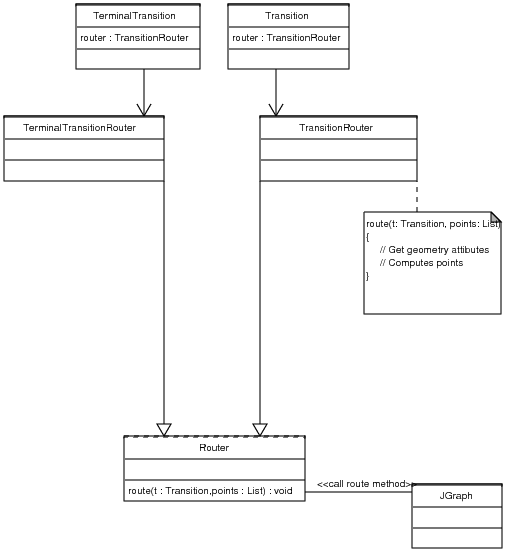
\includegraphics[width=16cm, height=20cm]{img/routing.png}
  \caption{Translation of geometric properties of transitions}
  \label{diaroute}
\end{figure}




\end{document}

